\documentclass{article}
\usepackage{blindtext} %creates some lorem ipsum for words
\usepackage{listings}
\usepackage{graphicx}
\title{Matt's CUDA CheatSheet (And \LaTeX\ practice)}
\date{2018\\ February}
\author{Matthew Hanley}

\begin{document}
\maketitle
\section{Basic Commands}

Copy memory:
\begin{lstlisting}
cudaMemcpy(void *dst, void *src, size_t count, cudaMemcpyKind)
\end{lstlisting}

Launch Kernel:
\begin{lstlisting}
my_kernel<<<dimGrid,dimBlock>>>(input-1, input-2)
\end{lstlisting}

\section{Lorem Ipsum}
\blindtext

\section{Figures and Graphics}
\blindtext
\begin{figure}[bh]
  \centering
  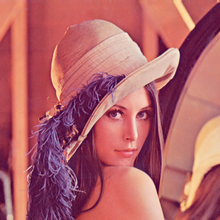
\includegraphics[scale=0.5]{girl}
  \caption{Scaled .png photo. Pretty neat.}
\end{figure}

\end{document}
